\documentclass[ngerman,10pt,a4paper,titlepage]{report}
\usepackage[T1]{fontenc}
\usepackage[left=1.5cm, right=1.5cm]{geometry}
\usepackage{graphicx}
\usepackage{babel}
\usepackage{hyperref}
\usepackage{fontspec}
\usepackage{setspace}
\usepackage{ragged2e}
\usepackage{listings}
\usepackage{xcolor}
\usepackage{tabularx}
\usepackage{tabto}
\usepackage{rotating}
\usepackage{lastpage}
\usepackage{fancyhdr}
\usepackage{csvsimple}


\definecolor{codegreen}{rgb}{0,0.6,0}
\definecolor{codegray}{rgb}{0.5,0.5,0.5}
\definecolor{codepurple}{rgb}{0.58,0,0.82}
\definecolor{backcolour}{rgb}{0.95,0.95,0.92}

\lstdefinestyle{mystyle}{
    backgroundcolor=\color{backcolour},   
	commentstyle=\color{codegreen},
	keywordstyle=\color{magenta},
	numberstyle=\tiny\color{codegray},
	stringstyle=\color{codepurple},
	basicstyle=\ttfamily\footnotesize,
	breakatwhitespace=false,         
	breaklines=true,                 
	captionpos=b,                    
	keepspaces=true,                 
	numbers=left,                    
	numbersep=5pt,                  
	showspaces=false,                
	showstringspaces=false,
	showtabs=false,                  
	tabsize=2
}
\lstset{style=mystyle}


\title{{\huge \textbf{Berechnungszeiten von PI\\ unter Verwendung von FreeRTOS und ESP32-S3}}}

\author{Nathanael Gubler}

\setmainfont{Inter}

\fancypagestyle{plain}{%
	\fancyhf{}%
	\fancyfoot[C]{\thepage\ von \pageref{LastPage}}%
	\fancyfoot[R]{Nathanael Gubler\\\textit{12.10.2024}}%
	\fancyhead[L]{Berechnungszeiten von Pi}
	\fancyhead[R]{Juventus Technikerschule}
	\renewcommand{\headrulewidth}{1.5pt}% Line at the header invisible
	\renewcommand{\footrulewidth}{0.4pt}% Line at the footer visible
}

\begin{document}
	\pagestyle{fancy}
	\lhead{Berechnungszeiten von Pi}
	\rhead{Juventus Technikerschule}
	\cfoot{\thepage \ von \pageref{LastPage}}
	\rfoot{Nathanael Gubler\\\textit{12.10.2024}}
	\renewcommand{\headrulewidth}{1.5pt}
	\renewcommand{\footrulewidth}{0.4pt}
	\addtolength{\headwidth}{-2cm}
	
	\doublespacing
	\maketitle
	\newgeometry{left=3cm, right=2cm,bottom=3.5cm, top=4cm}
	
	\tableofcontents
	\begingroup
	\let\clearpage\relax
	\listoffigures
	\listoftables
	\endgroup
	
	\chapter{Aufgabenstellung}
	\doublespacing
	Zur Berechnung der Kreiszahl $\pi$ sollten zwei Methoden unabhängig voneinander gestartet und deren Berechnungszeit für 5 Nachkommastellen verglichen werden können. Dies soll in C auf einem ESP32-S3 realisiert werden, unter Verwendung des FreeRtos Betriebssystems.\newline
	
	\textbf{Aufgabe:}
	\begin{itemize}
		\item Realisiere die Leibniz-Reihen-Berechnung in einem Task.
		\item Wähle einen weiteren Algorithmus aus dem Internet
		\item Realisiere den Algorithmus in einem weiteren Task.
		\item Schreibe einen Steuertask, der die zwei erstellten Tasks kontrolliert
	\end{itemize}
	Zudem waren das Verhalten bei Drücken von bestimmten Tasten sowie die Update Time des Displays vorgegeben.
	
	\chapter{Berechnungsmethoden}
	\section{Methode A: Madhava/Leibniz}\label{MethodeA}
	\doublespacing
	\justifying
	Diese Berechnungsmethode ist eine der rudimentären Methoden zur Berechnungsmethoden zur Approximation von Pi. Geläufig "Leibniz-Methode" genannt, wurde sie allerdings schon im 14. Jahrhundert vom indischen gelehrten Madhava von Sangamagrama (c. 1340 – c. 1425) beschrieben. Die kann als infinite Serie in folgender Form beschrieben werden:
	
	\begin{equation}\label{Madhava}
		\frac{\pi}{4} = \frac{1}{3} - \frac{1}{5} + \frac{1}{7} - \frac{1}{9} + \dots
	\end{equation}
	
	Durch den Wechsel zwischen Addition und Subtraktion entsteht ein hin- und her-\textit{\textacutedbl hüpfen\textacutedbl} um die Kreiszahl $\pi$ herum.
	
	\section{Methode B: Chudnovsky}\label{MethodeB}
	Eine alternative zu \ref{Madhava} stellt die vom den Brüdern David Volfovich Chudnovsk und Gregory Volfovich Chudnovsky entwickelte Methode dar. Diese ist eine Erweiterung einer vom indischen Mathematikers Srinivasa Ramanujan entwickelten Methode. Sie zeichnet sich durch eine sehr schnelle Konvergenz zu $\pi$ aus, mit jeweils mehreren Nachkommastellen pro Iteration:
	\begin{equation}\label{Chudnovsky}
		\frac{1}{\pi} = 12 \sum_{k=0}^\infty \frac{(-1)^{k}(6k)!(545140134 * k + 13591409)}{(3k)!(k!)^{3}640320^{3k + \frac{3}{2}}}
	\end{equation}
	Diese Formel kann umgeformt und vereinfacht weiter werden, sodass sie einfacher auf einem Prozessor zu realisieren ist. Im Internet existierte dazu bereits ein fertiger Code in Python, der allerdings rekursive Funktionsaufrufe beinhaltete:
	
	\lstinputlisting[language=Python, firstline=2]{chudnovsky.py}
	
	Im Laufe der Programmierarbeit führte der rekursive Ansatz jedoch zu instabilitäten auf dem ESP32. Daher wurde später ein Zwischenschritt in der Umformung verwendet:
	
	\begin{equation}\label{Chudnovsky_easy}
		\pi = \frac{426880 \sqrt{10005}}{13591409 + (545140134k + 13591409)*\sum_{k=1}^\infty \prod_{1}^{k}\frac{-(6k-1)(2j-1)(6j-5)}{10939058860032000k^{3}}}
	\end{equation}
	
	Diese Umformung führte zu mehr Stabilität. Jedoch entstanden extrem grossen Zahlen und darum auch extrem kleine Zwischenprodukte. Deswegen war der ESP32 bereits nach der zweiten Iteration überlastet. Das führte dazu, dass ein Schutzmechanismus eingebaut werden musste, der den Rechenprozess abbrach sobald zu kleine Zahlen entstanden.
	
	\chapter{Softwareaufbau}
	%\doublespacing
	Der Programmcode instanziert fünf verschiedene Task und vier Eventgroups, welche zur Synchronisation zwischen den Task dienen. Zudem waren globale Variablen zur Speicherung der aktuellen Daten sowie des Resultats nötig. Diese sind als Timestamps, kurz \textit{ts}, umgesetzt und beinhalten neben dem aktuellen Wert auch Anzahl Iterationen, start- und end-tick, sowie ob die Genauigkeit erreicht wurde.
	\section{Eventgroups}
	%\singlespacing
	\begin{itemize}
		\item {\large \textbf{Btn\_Eventgroup}}\\
		Die Tasteneingaben werden in diese Eventgroup geschrieben. Dabei wird zwischen kurzen und langen Tastendrücken unterschieden. Nach der Verarbeitung wird die Eventgroup wieder auf 0x00 gesetzt.
		\item {\large \textbf{Calc\_Eventgroup\_A/B}}\\
		Steuert die Zustände des jeweiligen Berechnungstasks (siehe \ref{TaskStates}).
		\item {\large \textbf{MethodInfo\_Eventgroup}}\\
		Zeigt, welche Berechnungsmethode vom Benutzer derzeit ausgewählt ist.
	\end{itemize}\newpage
	\section{Taskübersicht}
	\singlespacing
	\begin{itemize}
		\item {\large \textbf{ButtonTask}}
		\begin{itemize}
			\item Überprüft Tastenfunktion auf Änderungen und schreibt diese in Btn\_Eventgroup.
			\item Priorität:\tabto{5cm}\textbf{10}
			\item RAM:\tabto{5cm}\textbf{2*2048}
			\item Updatetime:\tabto{5cm}\textbf{\textit{ca.} 50ms}
			\item Schreibt Eventgroup:\tabto{5cm}\textbf{Btn\_Eventgroup}
		\end{itemize}
		\item {\large \textbf{LogicTask}}
		\begin{itemize}
			\item Wartet auf Änderungen von Btn\_Eventgroup und kontrolliert die Berechnungs-Eventgroups.
			\item Priorität:\tabto{5cm}\textbf{5}
			\item RAM:\tabto{5cm}\textbf{2*2048}
			\item Updatetime:\tabto{5cm}\textbf{undefiniert}
			\item Liest Eventgroup:\tabto{5cm}\textbf{Btn\_Eventgroup, MethodInfo\_Eventgroup}
			\item Schreibt Eventgroup:\tabto{5cm}\textbf{Calc\_Eventgroup\_A, Calc\_Eventgroup\_B,\\
				\tabto{5cm}MethodInfo\_Eventgroup}
		\end{itemize}
		\item {\large \textbf{DisplayTask}}
		\begin{itemize}
			\item Zeigt Text gemäss CalcTask Zuständen und globalen Daten an.
			\item Priorität:\tabto{5cm}\textbf{4}
			\item RAM:\tabto{5cm}\textbf{2*2048}
			\item Updatetime:\tabto{5cm}\textbf{\textit{ca.} 500ms}
			\item Liest Eventgroup:\tabto{5cm}\textbf{MethodInfo\_Eventgroup, Calc\_Eventgroup\_A,\\
				\tabto{5cm}Calc\_Eventgroup\_B,}
			\item Liest globale Variablen:\tabto{5cm}\textbf{g\_running\_ts\_A, g\_running\_ts\_B, g\_calc\_result\_A,\\
				\tabto{5cm}g\_calc\_result\_B}
			\item Schreibt Eventgroup:\tabto{5cm}\textbf{Calc\_Eventgroup\_A, Calc\_Eventgroup\_B}
		\end{itemize}
		\item {\large \textbf{CalcTaskA}}
		\begin{itemize}
			\item Berechnet iterativ gemäss der Madhava/Leibniz Methode (siehe \ref{MethodeA}) und überprüft das Resultat auf die gegebenen Grenzwerte.
			\item Priorität:\tabto{5cm}\textbf{2}
			\item RAM:\tabto{5cm}\textbf{8*2048}
			\item Updatetime:\tabto{5cm}\textbf{\textit{ca.} 1ms}
			\item Liest Eventgroup:\tabto{5cm}\textbf{Calc\_Eventgroup\_A}
			\item Schreibt Eventgroup:\tabto{5cm}\textbf{Calc\_Eventgroup\_A}
			\item Schreibt globale Variablen:\tabto{5cm}\textbf{g\_running\_ts\_A, g\_calc\_result\_A}
		\end{itemize}
		\item {\large \textbf{CalcTaskB}}
		\begin{itemize}
			\item Berechnet iterativ gemässe der Chudnovsky Methode (siehe \ref{MethodeB}) und überprüft das Resultat auf die gegebenen Grenzwerte.
			\item Priorität:\tabto{5cm}\textbf{2}
			\item RAM:\tabto{5cm}\textbf{8*2048}
			\item Updatetime:\tabto{5cm}\textbf{\textit{ca.} 1ms}
			\item Liest Eventgroup:\tabto{5cm}\textbf{Calc\_Eventgroup\_B}
			\item Schreibt Eventgroup:\tabto{5cm}\textbf{Calc\_Eventgroup\_B}
			\item Schreibt globale Variablen:\tabto{5cm}\textbf{g\_running\_ts\_B, g\_calc\_result\_B}
		\end{itemize}
	\end{itemize}
	\doublespacing
	Der DisplayTask nutzt die Funktion \textit{GetCurrTimestamp} um den jeweiligen Berechnungstask anzuhalten, die aktuellen Daten abzugreifen und dann wieder zu starten. Für die Anzeige der Resultate werden die Daten gelesen sobald die Genauigkeit erreicht wurde und der jeweilige Berechnungstask nicht das Resultat timestamp beschreibt. Abbildung \ref{fig:taskoverview} zeigt die Schnittstellen zwischen den Task sowie die Struktur des Timestamp structs.%\newpage
	\begin{sidewaysfigure}[h]
		\centering
		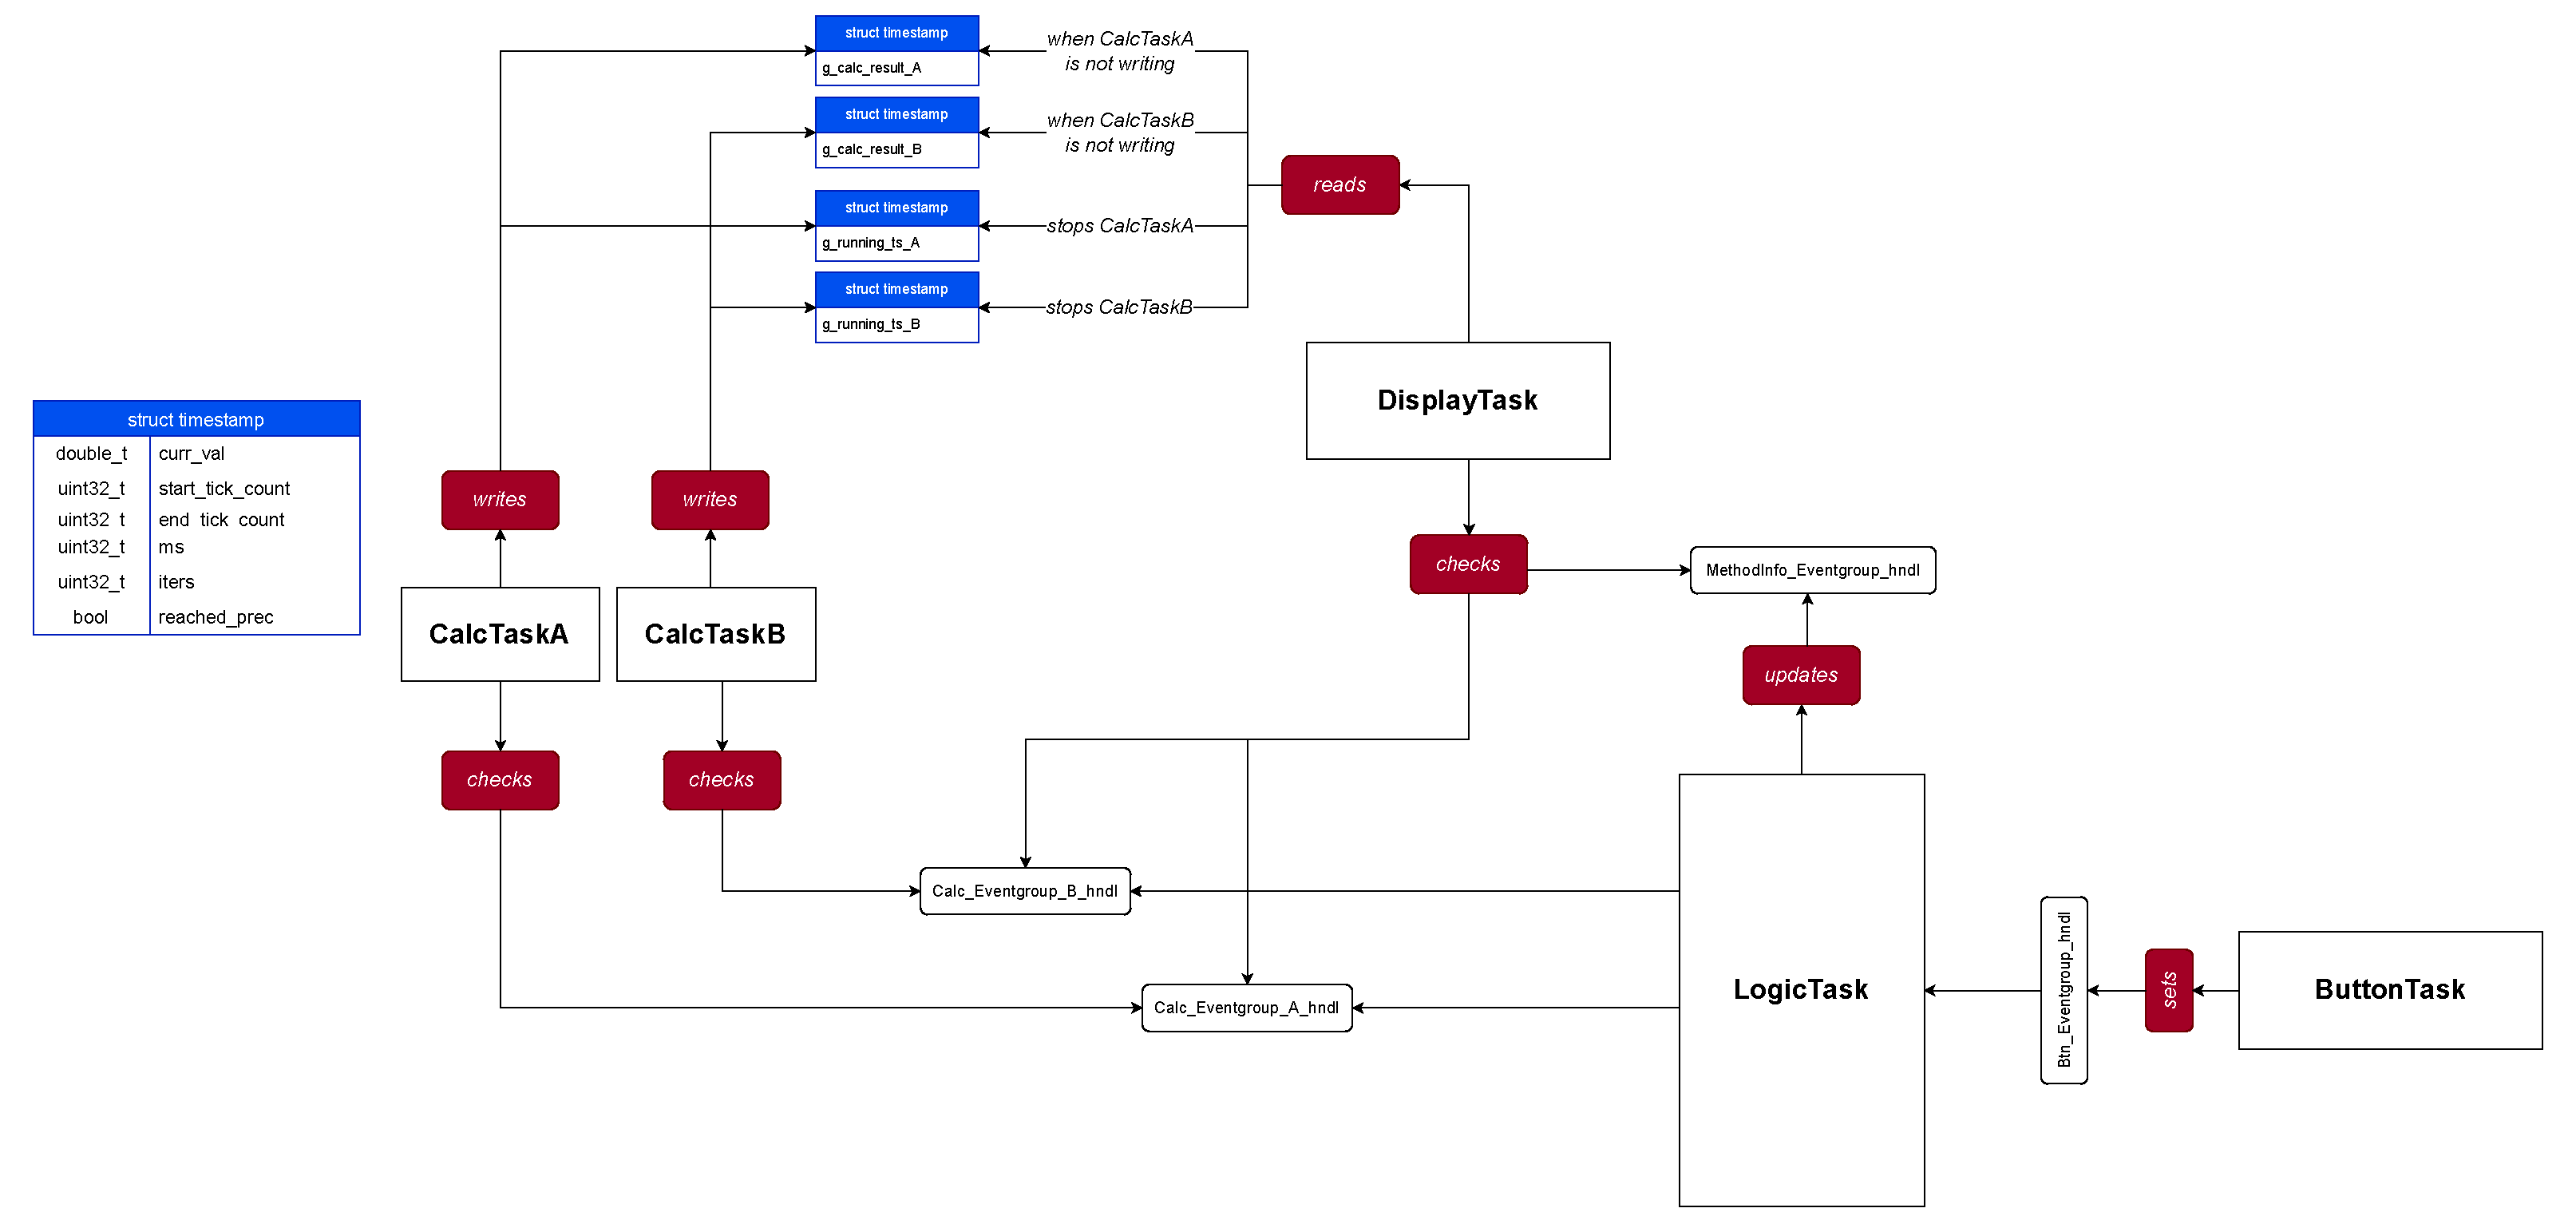
\includegraphics[width=1.1\linewidth]{diagrams/TaskOverview}
		\caption[Taskübersicht]{Die Tasks kommunizieren jeweils über Eventgroups oder globale Variabeln.}
		\label{fig:taskoverview}
	\end{sidewaysfigure}
	\section{Task states}\label{TaskStates}
	Die Berechnungstasks \textit{CalcTaskA} und \textit{CalcTaskB} prüfen in jedem loop, in welchem Zustand sie sich befinden. Dieser Zustand ist in der jeweiligen \textit{Calc\_Eventgroup} festgelegt. 
	Jeder Berechnungs-Task kann daher unabhängig voneinander die folgenden Zustände einnehmen:
	\begin{itemize}
		\item \textbf{STOPPING}:\tabto{3cm}Setzt die \textit{Calc\_Eventgroup} auf \textbf{STOPPED} und blockiert dann bis ein anderer Zustand in die Eventgroup gesetzt wird.
		\item \textbf{RESETTING}:\tabto{3cm}Setzt alle Werte des aktuellen sowie des Resultat-Timestamps zurück und setzt die \textit{Calc\_Eventgroup} auf \textbf{STOPPING}.
		\item \textbf{STARTING}:\tabto{3cm}Setzt den start tick count des aktuellen Timestamps zurück falls die Berechnung neu gestartet wurde. Setzt dann die \textit{Calc\_Eventgroup} auf \textbf{RUNNING}.
		\item \textbf{RUNNGING}:\tabto{3cm}Berechnet die nächste Iteration der jeweiligen Methode und überprüft dann fortlaufend, ob sich der aktuelle Wert innerhalb der gegebenen Grenzwerte befindet.
	\end{itemize}
	Zusätzlich gibt es noch den temporären Zustand \textbf{WRITING\_RESULT}, welcher allerdings nur zur Synchronisation dient. Abbildung \ref{fig:stateeventcalctasks} zeigt die Zustände und wie sie erreicht werden können.
	\begin{figure}
		\centering
		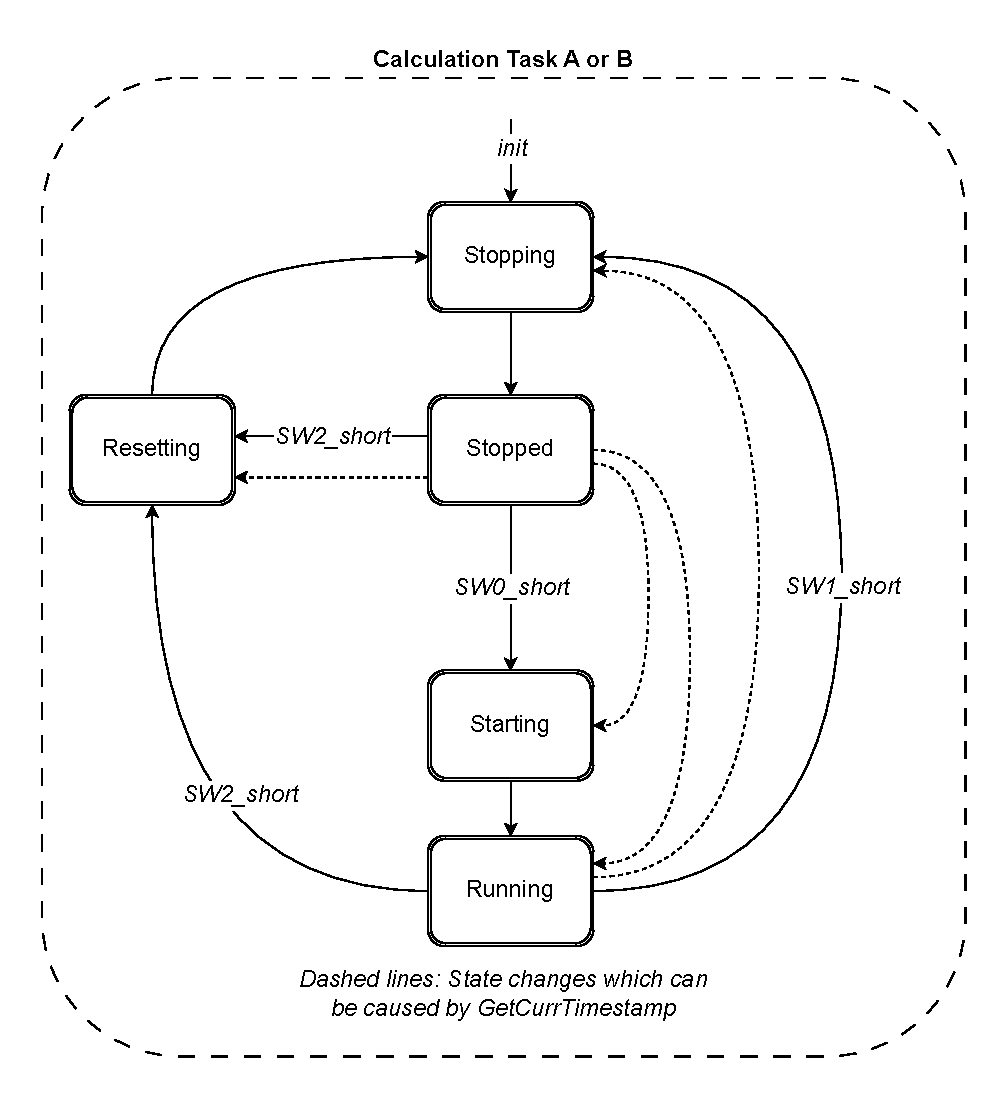
\includegraphics[width=0.7\linewidth]{diagrams/StateEvent_CalcTasks}
		\caption{State-Event Diagramm der Berechnungstasks. Übergänge ohne Text laufen automatisch ab.}
		\label{fig:stateeventcalctasks}
	\end{figure}
	Der LogicTask steuert den Wechsel zwischen den vom Benutzer ausgewählten Berechnungsmethode und leitet die Tasteneingaben jeweils um. Abbildung \ref{fig:stateeventlogictask} zeigt diese Zustände.
	\begin{figure}
		\centering
		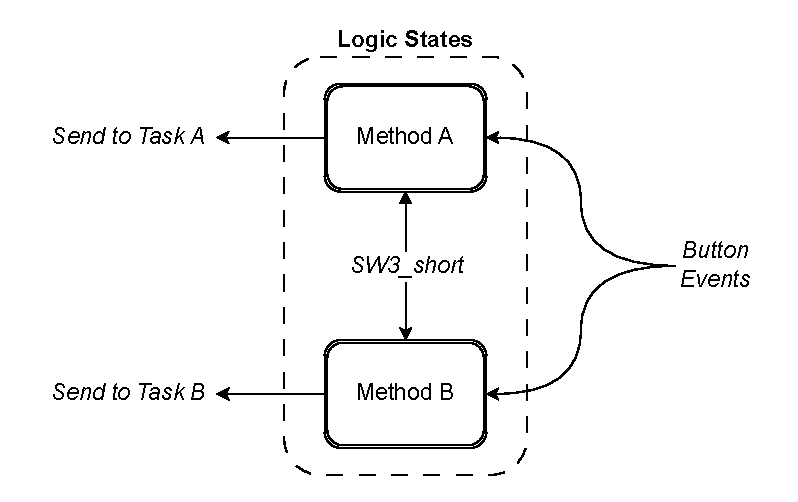
\includegraphics[width=0.7\linewidth]{diagrams/StateEvent_LogicTask}
		\caption{Die Zustände der Calc\_Eventgroups werden jeweils gemäss aktuell ausgewähltem Task und Tasteneingaben gesetzt.}
		\label{fig:stateeventlogictask}
	\end{figure}
	
	\chapter{Resultate}
	\section{Direktvergleich}\label{comparison}
	Es wurden mit beiden Methoden jeweils 10 Durchläufe gestartet und die Zeit bis die Methode fünf Nachkommastellen erreicht hatte gemessen. Tabelle \ref{ResultateA} zeigt die Resultate für Madhava-Leibniz.
	\begin{table}[h]
		\doublespacing
		\multicolumn{1}{c}{
		\begin{tabular}{c|c}\label{ResultateA}
			\multicolumn{2}{c}{{\large \textbf{Methode A}}}\\
			\textbf{Lauf} & \textbf{Zeit [ms]}% specify table head
			\csvreader[head to column names]{tests/runtimes_A.csv}{}% use head of csv as column names
			{\\\hline\csvcoli&\textbf{\csvcolii}}% specify your coloumns here
		\end{tabular}}
		\multicolumn{1}{c}{
			\begin{tabular}{c|c}\label{ResultateB}
				\multicolumn{2}{c}{{\large \textbf{Methode B}}}\\
				\textbf{Lauf} & \textbf{Zeit [ms]}% specify table head
				\csvreader[head to column names]{tests/runtimes_B.csv}{}% use head of csv as column names
				{\\\hline\csvcoli&\textbf{\csvcolii}}% specify your coloumns here
			\end{tabular}}
	\caption{Die Messresultate zeigen deutliche Unterschiede zwischen den Methoden.}
	\end{table}
	CalcTaskA, also die Madhava Methode, erreichte in Testläufen eine Genauigkeit von fünf Nachkommastellen nach \textbf{1741ms$\pm$9ms}.
	CalcTaskB, also die Chundnovsky Methode, erreichte in allen Testläufen bereits nach der ersten Iteration eine Genauigkeit von 12 Nachkommastellen und konnte daher gleich im ersten Tick erreicht werden. Dies führte dazu, dass für die Zeitberechnung eine Tick-Differenz von 0 entstand und daher auch ein Zeitunterschied von \textit{\textacutedbl0ms\textacutedbl}.
	\section{Interpretation der Messungen}
	Die Ergebnisse in \ref{comparison} zeigen zum einen die enorme Effizienzunterschiede zwischen den beiden Methoden: Während die Madhava Methode mit jeder Iteration länger um eine Ziffer hin- und her springt, hantiert die Chudnovsky Methode bereits mit der ersten Iteration mit sehr grossen Zahlen. Somit hat die letztere Methode den Vorteil, mit jeder Iteration mehrere Dutzend Stellen sehr effizient zu berechnen.\\Zudem lässt sich aus dem Geschwindigkeitsunterschied ableiten, dass ein Prozessor wie der ESP32 so aufgebaut ist, dass grosse Zahlen schneller verarbeitet werden als viele kleinere.
	%\bibliographystyle{abbrv}
	%\bibliography{biblio.bib}
	
\end{document}